\documentclass{beamer}
\usepackage[utf8]{inputenc}

\usetheme{Madrid}
\usecolortheme{default}
\usepackage{amsmath,amssymb,amsfonts,amsthm}
\usepackage{txfonts}
\usepackage{tkz-euclide}
\usepackage{listings}
\usepackage{adjustbox}
\usepackage{array}
\usepackage{tabularx}
\usepackage{gvv}
\usepackage{lmodern}
\usepackage{circuitikz}
\usepackage{tikz}
\usepackage{graphicx}

\setbeamertemplate{page number in head/foot}[totalframenumber]

\usepackage{tcolorbox}
\tcbuselibrary{minted,breakable,xparse,skins}



\definecolor{bg}{gray}{0.95}
\DeclareTCBListing{mintedbox}{O{}m!O{}}{%
  breakable=true,
  listing engine=minted,
  listing only,
  minted language=#2,
  minted style=default,
  minted options={%
    linenos,
    gobble=0,
    breaklines=true,
    breakafter=,,
    fontsize=\small,
    numbersep=8pt,
    #1},
  boxsep=0pt,
  left skip=0pt,
  right skip=0pt,
  left=25pt,
  right=0pt,
  top=3pt,
  bottom=3pt,
  arc=5pt,
  leftrule=0pt,
  rightrule=0pt,
  bottomrule=2pt,
  toprule=2pt,
  colback=bg,
  colframe=orange!70,
  enhanced,
  overlay={%
    \begin{tcbclipinterior}
    \fill[orange!20!white] (frame.south west) rectangle ([xshift=20pt]frame.north west);
    \end{tcbclipinterior}},
  #3,
}
\lstset{
    language=C,
    basicstyle=\ttfamily\small,
    keywordstyle=\color{blue},
    stringstyle=\color{orange},
    commentstyle=\color{green!60!black},
    numbers=left,
    numberstyle=\tiny\color{gray},
    breaklines=true,
    showstringspaces=false,
}
\begin{document}

\title 
{5.8.4}
\date{oct 4,2025}


\author 
{ADUDOTLA SRIVIDYA -EE25BTECH11006}






\frame{\titlepage}

\begin{frame}{Question}
The centre of the circle passing through $(0,0)$ and $(1,0)$ and touching the circle $x^2 +y^2 = 9$ is
\end{frame}

\begin{frame}{Solution}
    Let the required circle be represented as
\begin{align}
\vec{x}^{T}\vec{V}\vec{x} + 2\vec{u}^{T}\vec{x} + f = 0,
\label{eq:circle-general}
\end{align}
where $\vec{V} = \myvec{1 & 0 \\ 0 & 1} = \vec{I}$.

\textbf{Condition 1: Passing through $\vec{P}=\myvec{0\\0}$ and $\vec{Q}=\myvec{1\\0}$}

\begin{align}
\vec{P}^{T}\vec{V}\vec{P} + 2\vec{u}^{T}\vec{P} + f = 0, \label{eq:circle-P}\\
\vec{Q}^{T}\vec{V}\vec{Q} + 2\vec{u}^{T}\vec{Q} + f = 0. \label{eq:circle-Q}
\end{align}
\end{frame}

\begin{frame}{Solution}
    Subtracting (2) from (3),
\begin{align}
\brak{\vec{Q}^{T}\vec{V}\vec{Q} - \vec{P}^{T}\vec{V}\vec{P}} + 2\vec{u}^{T}\brak{\vec{Q} - \vec{P}} = 0. \label{eq:diff}
\end{align}
\end{frame}

\begin{frame}{Solution}
    \textbf{Condition 2: Touching the given circle}

The given circle is
\begin{align}
\vec{x}^{T}\vec{V}\vec{x} + 2\vec{u_1}^{T}\vec{x} + f_1 = 0,
\end{align}
where
\begin{align}
\vec{u_1} = \myvec{0\\0}, \quad f_1 = -9.
\end{align}

Hence,
\begin{align}
\vec{c_1} = -\vec{u_1} = \myvec{0\\0}, \quad r_1 = \sqrt{\vec{u_1}^{T}\vec{u_1} - f_1} = 3.
\end{align}

For the required circle,
\begin{align}
\vec{c_2} = -\vec{u}, \quad r_2 = \sqrt{\vec{u}^{T}\vec{u} - f}. \label{eq:c2r2}
\end{align}
\end{frame}

\begin{frame}{Solution}
    Since the circles touch each other internally,
\begin{align}
\norm{\vec{c_1} - \vec{c_2}} = r_1 - r_2. \label{eq:tangent}
\end{align}

Substitute (8) into (9):
\begin{align}
\norm{\vec{u}} = 3 - \sqrt{\vec{u}^{T}\vec{u} - f}. \label{eq:relation}
\end{align}

\textbf{Substitute condition from points}

From (2):
\begin{align}
\vec{P}^{T}\vec{V}\vec{P} + 2\vec{u}^{T}\vec{P} + f = 0 \implies f = -2\vec{u}^{T}\vec{P} - \vec{P}^{T}\vec{V}\vec{P}. \label{eq:f}
\end{align}
\end{frame}

\begin{frame}{Solution}
    Substitute (11) into (10):
\begin{align}
\norm{\vec{u}} = 3 - \sqrt{\vec{u}^{T}\vec{u} + 2\vec{u}^{T}\vec{P} + \vec{P}^{T}\vec{V}\vec{P}}.
\label{eq:u_equation}
\end{align}

From (4), we also have
\begin{align}
2\vec{u}^{T}\brak{\vec{Q} - \vec{P}} = -\brak{\vec{Q}^{T}\vec{V}\vec{Q} - \vec{P}^{T}\vec{V}\vec{P}}.
\label{eq:u_cond}
\end{align}

\textbf{Now substitute specific vectors}

\begin{align}
\vec{P} = \myvec{0\\0}, \quad \vec{Q} = \myvec{1\\0}.
\end{align}
\end{frame}

\begin{frame}{Solution}
    From (13),
\begin{align}
2\vec{u}^{T}\myvec{1\\0} = -\brak{1 - 0} \implies \vec{u}^{T}\myvec{1\\0} = -\frac{1}{2}.
\end{align}

Let $\vec{u} = \myvec{u_1\\u_2}$. Then
\begin{align}
u_1 = -\frac{1}{2}.
\end{align}

From (12), using $\vec{P} = \myvec{0\\0}$,
\begin{align}
\norm{\vec{u}} = 3 - \sqrt{\vec{u}^{T}\vec{u}}.
\end{align}
\end{frame}

\begin{frame}{Solution}
    Let $\sqrt{\vec{u}^{T}\vec{u}} = k$.
\begin{align}
k = 3 - k \implies 2k = 3 \implies k = \frac{3}{2}.
\end{align}
\begin{align}
\vec{u}^{T}\vec{u} = \frac{9}{4}.
\end{align}

Hence,
\begin{align}
u_1^2 + u_2^2 = \frac{9}{4}.
\end{align}
\end{frame}

\begin{frame}{Solution}
    Substitute $u_1 = -\frac{1}{2}$:
\begin{align}
\frac{1}{4} + u_2^2 = \frac{9}{4} \implies u_2^2 = 2.
\end{align}
\begin{align}
u_2 = \pm \sqrt{2}.
\end{align}


\textbf{Centre of the required circle:}
\begin{align}
\vec{c_2} = -\vec{u} = \myvec{\frac{1}{2} \\ -u_2} = 
\myvec{\frac{1}{2} \\ \mp \sqrt{2}}.
\end{align}
\end{frame}

\begin{frame}{Solution}
    \textbf{Hence, the two possible centres are:}
\begin{align}
\vec{c_2} = \myvec{\frac{1}{2} \\ \sqrt{2}} \quad \text{and} \quad
\vec{c_2} = \myvec{\frac{1}{2} \\ -\sqrt{2}}
\end{align}
\end{frame}

\begin{frame}[fragile]
\frametitle{Python,C,Python+C codes}
codes permalink
\end{frame}

\begin{frame}{Plot}
    \begin{figure}[h!]
    \centering
    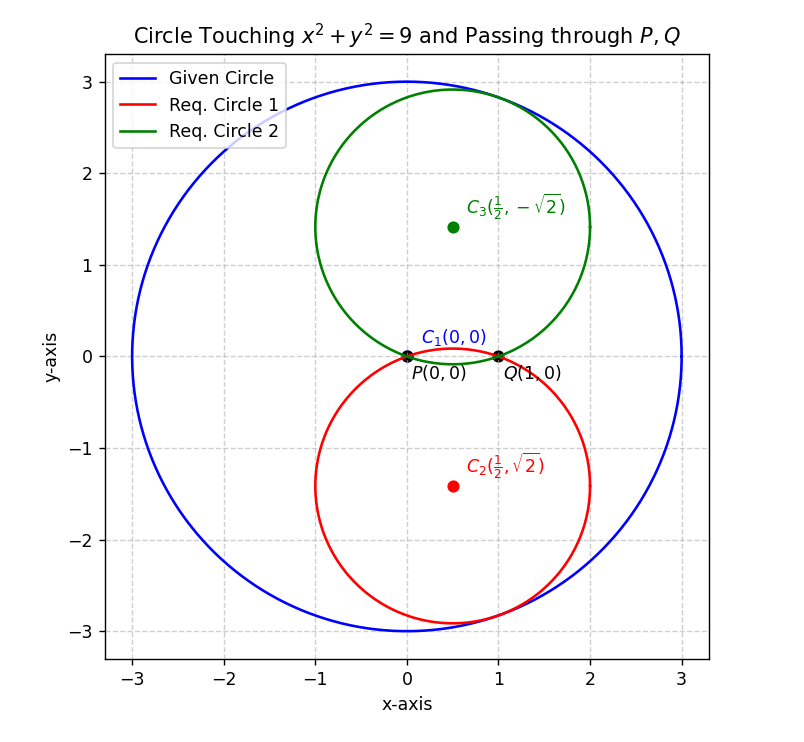
\includegraphics[height=0.5\textheight, keepaspectratio]{figs/fig.png}
    \label{figure_1}
\end{figure}
\end{frame}

\end{document}